\chapter{Realisierung}\label{AppendixRealisierung}

\section{HTML-Prototyp}

Der HTML-Prototyp ist im Verzeichnis «html-prototype» zu finden, dieser wurde
mit \textbf{Ember.js} und \textbf{SASS} umgesetzt.
Um den Prototypen zu starten muss \textbf{Node.js} und \textbf{Yarn} installiert sein.


\noindent
Den Prototypen kann man mit dem folgenden Kommando starten:

\begin{lstlisting}[language=bash,frame=single]
$ yarn && yarn start
\end{lstlisting}

\noindent
Danach kann der Prototyp über die URL \url{http://localhost:4200/} geöffnet werden.

\noindent
Folgende URLs sind verfügbar:

\begin{itemize}
  \tightlist{}
  \item{} \url{http://localhost:4200/}
  \item{} \url{http://localhost:4200/search}
  \item{} \url{http://localhost:4200/gig-detail}
  \item{} \url{http://localhost:4200/add-gig}
  \item{} \url{http://localhost:4200/login}
  \item{} \url{http://localhost:4200/register}
\end{itemize}

\clearpage
\section{Projekt Setup}

Die Initialisierung des Projekts wurde mit der Phoenix Framework «Umbrella»
Struktur erstellt.

\begin{lstlisting}[language=bash,frame=single]
$ mix phx.new gigpillar --umbrella
\end{lstlisting}

Die Umbrella Struktur trennt die Applikation in kleinere Teilapplikationen,
dies ermöglicht eine klarere Trennung zwischen der Webapplikation und der Businesslogik.

\noindent
Erläuterung der Projekt/Dateistruktur:

\begin{lstlisting}[frame=single]
/apps/gigpillar/
\end{lstlisting}
Die Gigpillar Grundapplikation

\begin{lstlisting}[frame=single]
# Die Gigpillar Webapplikation
/apps/gigpillar_web/
# Applikations{\"u}bergreifende Konfigurationsfiles
/config/
# Die Projektdokumentation
/doc/
# Der HTML-Prototyp
/html-prototype/
# Die Dockerkonfiguration f{\"u}r die Entwicklungsumgebung
/docker-compose.yml
# Die applikationsubergreiffenden Abhangigkeiten
/mix.exs
\end{lstlisting}

\section{Dependency Management}

Für das Dependency Management, wurde ein Bot eingerichtet, der
Benachrichtigungen, bzw. Pull-Requests, bei Updates zustellt.

Für das Projekt wurde der Bot «Dependabot»\footnote{\url{https://github.com/marketplace/dependabot}} ausgewählt, da diser Elixir sowie JavaScript Abhängigkeiten unterstützt.

Durch die Benützung des Dependabot, können während der Entwicklung des Projektes
die Software Abhängigkeiten jederzeit auf dem neusten Stand gehalten werden.

\clearpage
\section{Datenbankschema}

\subsubsection{Alle Entitäten}
Alle «created\_at» Felder wurden nach «inserted\_at» umbenannt, da dies die
Standardbenennung des Phoenix Frameworks ist.

\subsubsection{User}
Der Benutzer Entität wurde das Feld «password» nach «password\_hash» umbenannt,
damit klar ist, dass nicht ein Passwort sondern nur ein Hash abgespeichert wird.

\subsubsection{Genre}
Der Genre Entität sind im Konzept die Datumsfelder «update\_at» und «inserted\_at»
vergessen gegangen und wurden in der Realisierung nachgeführt.

\subsubsection{Gig}
In der Gig Entität wurden drei weitere Felder hinzugefügt.
Die Felder «uuid» und «picture» dienen dazu, die beim Erfassen sowie
Bearbeiten eines Gigs hochgeladenen Bilder zu identifizieren.
Das zusätzliche Feld «tickets» ermöglicht es, beim Erfassen eines Gigs
einen Link zum Ticketvorverkauf zu hinterlegen.

\subsubsection{Location}
Die Location Entität erhielt bei der Realisierung zwei neue Felder,
«address» für die Adresse der Location und
«google\_place\_id» um die Referenz der Google API zu erhalten.

\clearpage
\subsection{Finales Schema}

\begin{figure}[!htb]
  \centering
  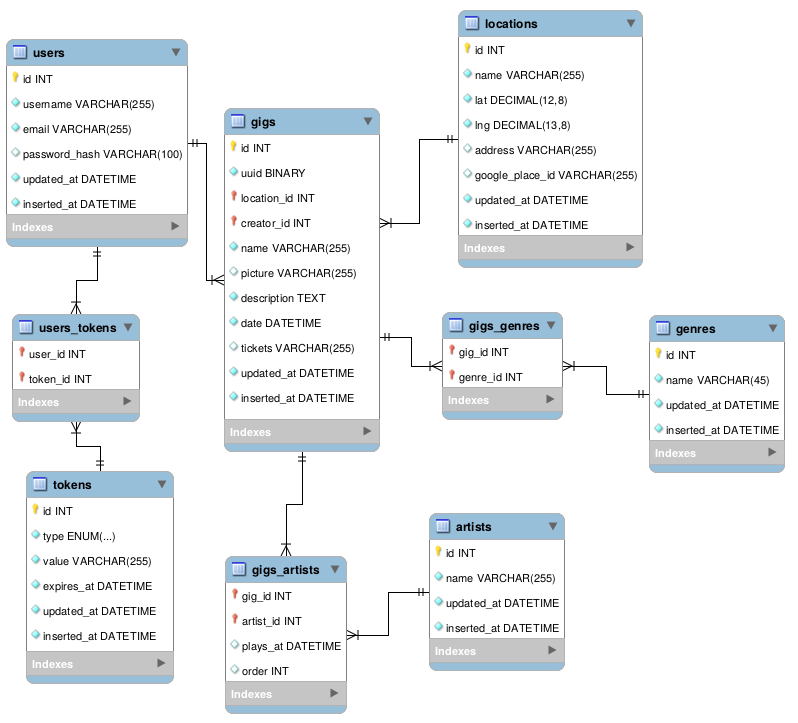
\includegraphics[width=0.95\textwidth]{realisierung/erd.png}
  \caption{Realisierung: Entity Relationship Diagram}
\end{figure}

\clearpage
\section{Berechtigungssystem}

Das Bearbeiten von Gigs wurde so eingeschränkt, dass nur angemeldete Benutzer Gigs erstellen dürfen und Benutzer nur eigene Gigs bearbeiten können.

Dazu wurde die Library «Canary»\footnote{\url{https://github.com/cpjk/canary}} verwendet. In der Datei «apps/gigpillar/lib/abilities.ex» wurden die Berechtigungen wie gefolgt umgesetzt:

\lstinputlisting[language=elixir,frame=single]{../apps/gigpillar/lib/abilities.ex}

\clearpage
\section{Location Autocomplete}

Das Location Autocomplete Feld wurde mit der «Google Place API»\footnote{\url{https://developers.google.com/places/web-service/autocomplete}} umgesetzt.

Die verwendete Library «google-api-elixir-client» implementiert die
Autocomplete API, jedoch fehlte noch die entsprechende Zusatzfunktion um
weitere Details, wie die geographischen Koordinaten, Adresse, etc., zu den gefundenen Locations abzufragen.

Die API um Details abzufragen wurden im Rahmen von diesem Projekt umgesetzt
und zurück an das originale Projekt beigesteuert.

Ausserdem musste eine Abhängigkeit auf den aktuellsten Stand gebracht werden.

Die beiden Beiträge für die Library sind auf Github zu finden:

\begin{itemize}
  \item{} \url{https://github.com/seanabrahams/google-api-elixir-client/pull/10/files}
  \item{} \url{https://github.com/seanabrahams/google-api-elixir-client/pull/11/files}
\end{itemize}

\clearpage
\section{HTML Erweiterungen}

Während der Entwicklung des Projektes, wurden einige spezielle HTML-Elemente
definiert. Diese Elemente wurden mit \textbf{LitElement}\footnote{\url{https://lit-element.polymer-project.org/}}
umgesetzt, und bieten gegenüber den Standard HTML-Elementen eigens definierte
Verhaltensweisen.

\subsubsection{<search-box>}

Das \textbf{<search-box>} Element wird für die Suche sowie diverse
Autocomplete-Elemente verwendet. Stylistisch sieht die Suchbox aus wie
ein normales Texteingabefeld, mit einer kleiner Lupe als Symbol.\\
\\
\noindent{}Beispiel:

\begin{lstlisting}[language=html,frame=single]
<search-box
  inputId="suche"
  src="/api/autocomplete"
  name="suche"
  placeholder="Suche..."
  value="Suchbegriff"
  debounce-time="300"></search-box>
\end{lstlisting}

\noindent{}Attribute:
\begin{itemize}
  \tightlist{}
  \item{} \textbf{inputId:} Das \textbf{id} Attribut für das Input Element innerhalb der Suchbox, z.B. im Zusammenhang mit einem \textbf{<label>} Element.
  \item{} \textbf{src:} URL für die Datenabfrage, bei Eingaben in das Textfeld wird jeweils eine \textbf{HTTP} Abfrage ausgelöst und ein \textbf{search-result} Ereignis ausgelöst.
  \item{} \textbf{name:} Der Name des Form-Elements.
  \item{} \textbf{placeholder:} Platzhaltertext welcher dargestellt wird wenn das Textfeld leer ist.
  \item{} \textbf{value:} Der Wert, welcher mit dem HTML-Formular mitgeschickt wird.
  \item{} \textbf{debounce-time:} Zeit in Millisekunden die mindestens vergehen muss, bevor eine neue Abfrage an den Server geschickt wird.
\end{itemize}

\subsubsection{<with-dropdown>}

Mit dem \textbf{<with-dropdown>} Element können Dropdowns realisiert werden.
Elemente mit dem Attribut \textbf{slot="dropdown"} werden initial nicht dargestellt.
Wird ein Element innerhalb des \textbf{<with-dropdown>} Element fokussiert, so werden die mit \textbf{slot="dropdown"} gekennzeichneten Elemente innerhalb eines Dropdown-Elements dargestellt.\\
\\
\noindent{}Beispiel:

\begin{lstlisting}[language=html,frame=single]
<with-dropdown>
  <input type="text">
  <ul slot="dropdown">
    <li>Lorem</li>
    <li>Ipsum</li>
  </ul>
</with-dropdown>
\end{lstlisting}

\subsubsection{<location-input>}

Das \textbf{<location-input>} Element wird verwendet um für einen Gig eine
Location auszuwählen. Es repräsentiert ein Suchfeld, das eine Abfrage über die
Google Place API macht. Wird eine Location ausgewählt, wird das Suchfeld durch
einen Text sowie Button ersetzt. Der Text beinhaltet den Namen der Location und
der Button ermöglicht es, die ausgewählte Location mit einer Neuen zu ersetzen.\\
\\
\noindent{}Beispiel:

\begin{lstlisting}[language=html,frame=single]
<location-input
  inputId="gig_location"
  name="gig[location]"
  location="{
    "name": "Dachstock",
    "google_place_id": "ChIJ-SskKr45jkcRPqmGB-ZGsRE"
  }"></location-input>
\end{lstlisting}

\noindent{}Attribute:
\begin{itemize}
  \tightlist{}
  \item{} \textbf{inputId:} Das \textbf{id} Attribut für das Input Element innerhalb des Location-Input, z.B. im Zusammenhang mit einem \textbf{<label>} Element.
  \item{} \textbf{name:} Der Name des Form-Elements.
  \item{} \textbf{location:} Ein \textbf{JSON}-Objekt einer Location, bestehend aus \textbf{name} und einer \textbf{id} oder \textbf{google\_place\_id}.
\end{itemize}

\subsubsection{<picture-input>}

Als verbessertes File-Input, wurde ein Ersatz für ein
\textbf{<input type=file>} Element geschrieben. Das \textbf{<picture-input>}
Element funktioniert als kompatibler Ersatz und bietet die selbe Funktionalität an.
Der Hauptunterschied liegt in der Darstellung, so wird beim \textbf{<picture-input>}
jederzeit eine Vorschau für das ausgewählte Bild dargestellt.\\
\\
\noindent{}Beispiel:

\begin{lstlisting}[language=html,frame=single]
<picture-input
  inputId="gig-picture"
  name="gig[picture]"
  value="http://example.com/my-picture.png"></picture-input>
\end{lstlisting}

\noindent{}Attribute:
\begin{itemize}
  \tightlist{}
  \item{} \textbf{inputId:} Das \textbf{id} Attribut für das Input Element innerhalb des Picture-Input, z.B. im Zusammenhang mit einem \textbf{<label>} Element.
  \item{} \textbf{name:} Der Name des Form-Elements.
  \item{} \textbf{value:} URL oder Datei des ausgewählten Bildes.
\end{itemize}

\clearpage
\subsubsection{<datetime-input>}

Das \textbf{<datetime-input>} Element kombiniert ein \textbf{<input type=date>}
mit einem \textbf{<input type=time>} zu einem Feld zusammen.
\\
\noindent{}Beispiel:

\begin{lstlisting}[language=html,frame=single]
<datetime-input
  inputId="datetime"
  dateLabel="Datum"
  timeLabel="Uhrzeit"
  name="datetime"
  value="2019-05-14T17:50:14.608Z"></datetime-input>
\end{lstlisting}

\noindent{}Attribute:
\begin{itemize}
  \tightlist{}
  \item{} \textbf{inputId:} Das \textbf{id} Attribut für das Input Element innerhalb des Datetime-Input, z.B. im Zusammenhang mit einem \textbf{<label>} Element.
  \item{} \textbf{dateLabel:} Beschriftung für das Datumsfeld.
  \item{} \textbf{timeLabel:} Beschriftung für das Zeitfeld.
  \item{} \textbf{name:} Der Name des Form-Elements.
  \item{} \textbf{value:} Datum mit Zeit im \textbf{ISO 8601}\footnote{\url{https://de.wikipedia.org/wiki/ISO_8601}} Format.
\end{itemize}

\subsubsection{<artists-input>}

Das \textbf{<artists-input>} ist ein spezifisches Feld für das Erfassen von
Künstlern für ein Konzert. Es Sucht über den Server bereits existierende
Künstler, und bietet diese zur Auswahl an. Zusätzlich kann für jeden
ausgewählten Künstler eine Zeit angegeben werden, an welcher deren Auftritt
stattfindet.\\
\\
\noindent{}Beispiel:

\begin{lstlisting}[language=html,frame=single]
<artists-input
  inputId="artists"
  name="gig[artists]"
  placeholder="K&uuml;nstler suchen..."
  value="[
    {"id":42,"name":"Parkway Drive","plays_at":"23:00"},
    {"id":23,"name":"The Ghost Inside","plays_at":"21:00"}
  ]"></artists-input>
\end{lstlisting}

\noindent{}Attribute:
\begin{itemize}
  \tightlist{}
  \item{} \textbf{inputId:} Das \textbf{id} Attribut für das Input Element innerhalb des Artists-Input, z.B. im Zusammenhang mit einem \textbf{<label>} Element.
  \item{} \textbf{name:} Der Name des Form-Elements.
  \item{} \textbf{placeholder:} Platzhalter für das Suchfeld.
  \item{} \textbf{value:} Eine Liste von \textbf{JSON}-Objekten der einem Gig assozierten Künstler.
\end{itemize}

\clearpage
\section{Asset Optimierungen}

Für die Produktionsumgebung, wurden diverse Optimierungen vorgenommen:

\begin{itemize}
  \tightlist{}
  \item{} Terser Plugin um JavaScript Code zu optimieren.
  \item{} Plugin um Funktionen zu deduplizieren.
  \item{} HTML Minifier Plugin um HTML innerhalb von JavaScript zu optimieren.
  \item{} Imagemin Plugin um Bilder auf Dateigrösse zu optimieren.
  \item{} CSS Optimierungsplugin
  \item{} Zopfli Kompression
  \item{} Brotli Kompression
\end{itemize}

\begin{longtable}[]{@{}llr@{}}
  \toprule
  \textbf{Optimierungen} & \textbf{Datei} & \textbf{Grösse}\tabularnewline
  \midrule
  Keine & app.js & 1000 KiB\tabularnewline
  Produktionsmodus & app.js & 397 KiB\tabularnewline
  ” und Terser Plugin & app.js & 125 KiB\tabularnewline
  ” und Funktionsdeduplizierung & app.js & 123 KiB\tabularnewline
  ” und HTML Minifier & app.js & 122 KiB\tabularnewline
  ” mit Zopfli & app.js.gz & 25.2 KiB\tabularnewline
  ” mit Brotli & app.js.br & 23.0 KiB\tabularnewline
  \bottomrule
  \caption{JavaScript Optimierungen}
\end{longtable}

\begin{longtable}[]{@{}llr@{}}
  \toprule
  \textbf{Optimierungen} & \textbf{Datei} & \textbf{Grösse}\tabularnewline
  \midrule
  Keine & app.css & 10.5 KiB\tabularnewline
  Produktionsmodus & app.css & 10.5 KiB\tabularnewline
  ” und CSS Optimierungsplugin & app.css & 8.58 KiB\tabularnewline
  \bottomrule
  \caption{CSS Optimierungen}
\end{longtable}

\begin{longtable}[]{@{}llr@{}}
  \toprule
  \textbf{Optimierungen} & \textbf{Datei} & \textbf{Grösse}\tabularnewline
  \midrule
  Keine & background-1.jpg & 1.79 MiB\tabularnewline
  Produktionsmodus & background-1.jpg & 1.79 MiB\tabularnewline
  ” und Imagemin (Qualität 75) & background-1.jpg & 278 KiB\tabularnewline
  \bottomrule
  \caption{Bilder Optimierungen}
\end{longtable}

\clearpage
\section{File Upload}

- minio
- exaws (document deps problem/override)
- resizing
- uuid
- asset host config

\section{Openstreetmap}

- calc

\clearpage
\section{Probleme}

\clearpage
\section{Offene Punkte}

\clearpage
\section{Tests}

\section{Auswertung}
